\section{Diagrama de Despliegue}

A continuación se describe la topología del sistema mediante un diagrama de despliegue, el cual muestra la estructura de los elementos de hardware y el software utilizado por cada uno de estos, así como las relaciones presentes entre los elementos y la forma en que se comunican entre ellos.

\begin{figure}[h]
	\centering
		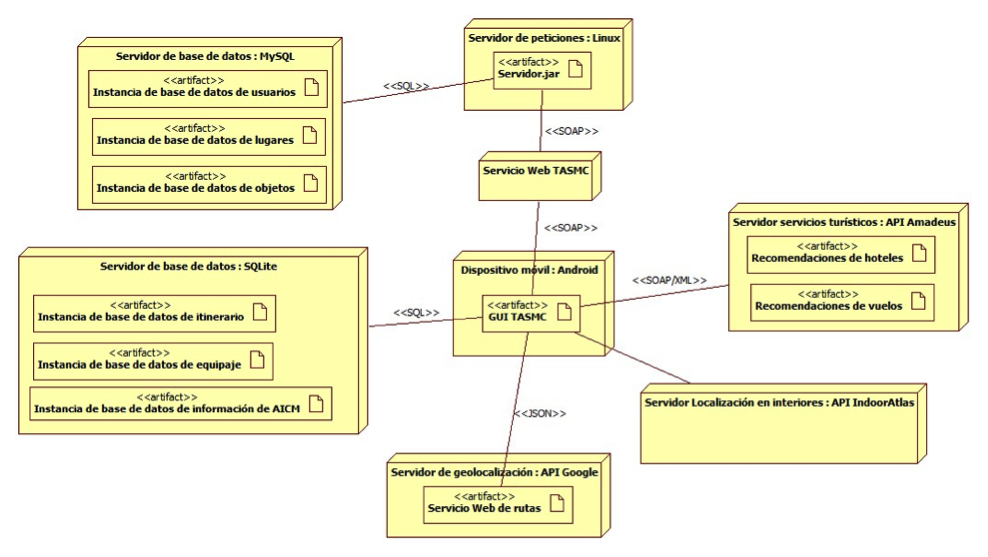
\includegraphics[width=1\textwidth]{Figuras/diagramaDespliegue.png}
		\rule{30em}{0.5pt}
	\caption[Diagrama de Despliegue]{Diagrama de Despliegue}
	\label{fig:diagramaDespliegue}
\end{figure}

El sistema consta de 8 elementos:

\begin{enumerate}
	\item Dispositivo móvil de Android.
	\item Servidor de peticiones Linux.
	\item Servidor de base de datos MySQL.
	\item Servidor de base de datos SQLite.
	\item Servidor de geolocalización Google.
	\item Servidor de localización en interiores IndoorAtlas.
	\item Servidor de servicios turísticos Amadeus.
	\item Servicio web TASMC.
\end{enumerate}

Estos dispositivos interactúan entre sí de la siguiente manera: 

El dispositivo móvil a través de la Interfaz Grafica de Usuario, manda a llamar mediante consultas SQL el servidor de base de datos de SQLite para obtener instancias de equipaje, itinerario e información del AICM, se envía una petición al Servidor de Geolocalización en formato JSON y llama el Servicio Web de Rutas, además de solicitar al Servidor de servicios turísticos mediante una intercambio SOAP/XML recomendaciones de hoteles y vuelos y finalmente la interacción a través de SOAP con el Servicio Web propio de TASMC que estará conectado con el servidor que se comunica con el Servidor de base de datos MySQL  que recibe peticiones SQL y busca instancias de usuarios, lugares y objetos que van a ser gestionados por el administrador del sistema y donde quedan registrados los lugares que serán representados en la interacción del dispositivo móvil con el servidor de localización en interiores IndoorAtlas.
